% ============================================================
%  TESIS: Automatización de un sistema fotoacústico
%         para la caracterización de líquidos
%  Autor  : Zarco Hernández Evandher Joel
%  Asesor : Dr. Arturo Ronquillo Arvizu
%  UNAM - Facultad de Ingeniería / ICAT
% ============================================================

\documentclass[12pt, letterpaper, oneside]{report}

% ── Codificación y lenguaje ──────────────────────────────────
\usepackage[utf8]{inputenc}
\usepackage[T1]{fontenc}
\usepackage[spanish, mexico]{babel}

% ── Tipografía ───────────────────────────────────────────────
\usepackage{lmodern}           % fuente Latin Modern (profesional, escalable)
\usepackage{microtype}         % mejora tipografía, reduce overfull hbox

% ── Márgenes (norma UNAM FI: izq 3cm, resto 2.5cm) ──────────
\usepackage[
  left   = 3cm,
  right  = 2.5cm,
  top    = 2.5cm,
  bottom = 2.5cm
]{geometry}

% ── Interlineado ─────────────────────────────────────────────
\usepackage{setspace}
\onehalfspacing                % 1.5 interlineado estándar

% ── Gráficas e imágenes ──────────────────────────────────────
\usepackage{graphicx}
\usepackage{float}
\graphicspath{{./figuras/}{./figuras/celda/}}

% ── Matemáticas ──────────────────────────────────────────────
\usepackage{amsmath, amssymb, amsfonts}
\providecommand{\diameter}{\ensuremath{\varnothing}}
\usepackage{siunitx}           % unidades SI: \SI{10}{\kilo\hertz}

% ── Código fuente ────────────────────────────────────────────
\usepackage{listings}
\usepackage{xcolor}

\lstdefinestyle{pythonstyle}{
  language     = Python,
  basicstyle   = \ttfamily\small,
  keywordstyle = \color{blue}\bfseries,
  commentstyle = \color{gray},
  stringstyle  = \color{orange!80!black},
  numbers      = left,
  numberstyle  = \tiny\color{gray},
  frame        = single,
  breaklines   = true,
  captionpos   = b
}
\lstset{style=pythonstyle}

% ── Tablas ───────────────────────────────────────────────────
\usepackage{booktabs}          % líneas profesionales
\usepackage{multirow}
\usepackage{tabularx}
\usepackage{array}

% ── Hipervínculos y referencias ──────────────────────────────
\usepackage[
  colorlinks = true,
  linkcolor  = black,
  citecolor  = blue,
  urlcolor   = blue
]{hyperref}
\usepackage[spanish]{cleveref} % \cref{fig:x} → "figura 1"
\crefname{table}{tabla}{tablas}
\Crefname{table}{Tabla}{Tablas}
\crefname{section}{sección}{secciones}
\Crefname{section}{Sección}{Secciones}
\crefname{lstlisting}{listado}{listados}
\Crefname{lstlisting}{Listado}{Listados}
\crefname{chapter}{capítulo}{capítulos}
\Crefname{chapter}{Capítulo}{Capítulos}
\crefname{appendix}{apéndice}{apéndices}
\Crefname{appendix}{Apéndice}{Apéndices}

% ── Bibliografía ─────────────────────────────────────────────
\usepackage{csquotes}          % requerido por biblatex con babel
\usepackage[
  backend  = biber,
  style    = ieee,
  sorting  = none
]{biblatex}
\addbibresource{referencias.bib}

% ── Encabezados y pies de página ─────────────────────────────
\usepackage{fancyhdr}
\pagestyle{fancy}
\fancyhf{}
\fancyhead[L]{\small\leftmark}
\fancyhead[R]{\small\thepage}
\renewcommand{\headrulewidth}{0.4pt}
\setlength{\headheight}{15pt}

% ── TikZ (para las líneas decorativas de la portada) ─────────
\usepackage{tikz}
\usepackage{eso-pic}           % para elementos en posición absoluta

% ── Otros útiles ─────────────────────────────────────────────
\usepackage{caption}
\usepackage{subcaption}
\usepackage{enumitem}
\usepackage{pdfpages}          % para incluir PDFs externos si es necesario

% ============================================================
%  DOCUMENTO
% ============================================================
\begin{document}

% ── Numeración romana para las páginas preliminares ──────────
\pagenumbering{roman}
\pagestyle{empty}

% ── PORTADA ──────────────────────────────────────────────────
% ============================================================
%  PORTADA — UNAM Facultad de Ingeniería
% ============================================================

\newgeometry{left=1.5cm, right=1.5cm, top=2cm, bottom=2cm}
\begin{titlepage}
\thispagestyle{empty}   %

% ── Líneas verticales──
\begin{tikzpicture}[remember picture, overlay]
\draw[line width=3pt]
    ([xshift=2cm, yshift=-6.25cm]current page.north west)
    -- ([xshift=2cm, yshift=7.5cm]current page.south west);
\draw[line width=1pt]
    ([xshift=2.5cm, yshift=-5cm]current page.north west)
    -- ([xshift=2.5cm, yshift=7.5cm]current page.south west);
\end{tikzpicture}

% ── Columna logos │ Columna texto ────────────────────────────
%Columna izquierda
\noindent
\begin{minipage}[c][0.98\textheight][s]{5cm}
  \centering
  
\includegraphics[width=4.8cm]{escudo_unam}
  \vfill
  
\includegraphics[width=4cm]{escudo_fi}
\end{minipage}%
%espacio entre columnas
\hspace{1cm}%
%Columna derecha
\begin{minipage}[c][0.98\textheight][s]{\dimexpr\textwidth -6 cm\relax}
  \centering

  {\normalsize\bfseries\underline{UNIVERSIDAD NACIONAL AUTÓNOMA DE MÉXICO}}

  \vspace{0.5cm}

  {\normalsize\bfseries FACULTAD DE INGENIERÍA}

  \vspace{3cm}

  {\large\bfseries
    Automatización de un sistema fotoacústico\\[6pt]
    para la caracterización de líquidos}

  \vspace{3cm}

  {\normalsize\bfseries T\,E\,S\,I\,S}\\[6pt]
  {\small Que para obtener el título de}\\[6pt]
  {\normalsize\bfseries Ingeniero Mecatrónico}   %

  \vspace{2.5cm}

  {\normalsize\bfseries
    P\enspace R\enspace E\enspace S\enspace E\enspace N\enspace T\enspace A}

  \vspace{0.5cm}

  {\normalsize Zarco Hernandez Evandher Joel}             % 

  \vspace{2.5cm}

  {\normalsize\bfseries DIRECTOR(A) DE TESIS}

  \vspace{0.4cm}

  {\normalsize Dr. Ronquillo Arvizu Arturo}

  \vfill

  \begin{flushright}
    {\small Ciudad Universitaria, Cd. Mx., 2026}
  \end{flushright}

\end{minipage}

\end{titlepage}
\restoregeometry


% ── PÁGINAS PRELIMINARES ─────────────────────────────────────
\newpage
% ============================================================
%  DEDICATORIA  (opcional)
% ============================================================
\chapter*{}
\vspace*{\fill}
\begin{flushright}
  \textit{[Dedicatoria]}
\end{flushright}
\vspace*{\fill}
   % opcional, comenta si no quieres

\newpage
% ============================================================
%  AGRADECIMIENTOS
% ============================================================
\chapter*{Agradecimientos}
\addcontentsline{toc}{chapter}{Agradecimientos}

Al M. en C. Arturo Ronquillo Arvizu, director de esta tesis, por
haberme abierto las puertas del laboratorio, por la confianza de dejarme
intervenir un arreglo experimental en uso, y por la paciencia con que
acompañó un trabajo que avanzó a base de sesiones cortas y contratiempos
largos.

Al Laboratorio de Fotofísica y Películas Delgadas del Instituto de
Ciencias Aplicadas y Tecnología, por el espacio, el equipo y el tiempo de
instrumento sin los cuales este trabajo no habría sido posible.

A Luis Pablo Rangel Mendieta, cuya celda fotoacústica e hidrófono son el
arreglo sobre el que se construyó esta automatización. Buena parte de lo
que aquí se reporta descansa en lo que él dejó hecho.

A la Universidad Nacional Autónoma de México y a la Facultad de
Ingeniería, por una formación que fue exigente en el mejor sentido de la
palabra.

A mis padres, a mis abuelos y a mis tíos y tías, por un apoyo que nunca
estuvo condicionado a que las cosas salieran bien. Lo que soy y lo que
pude terminar se lo debo a ellos.

A mis amigos, que me alentaron a seguir adelante y que estuvieron
presentes en los peores momentos. Terminar esto solo habría sido mucho
más difícil, y bastante menos llevadero.


\newpage
\tableofcontents
\newpage
\listoffigures
\newpage
\listoftables

% ── RESUMEN ──────────────────────────────────────────────────
\newpage
% ============================================================
% RESUMEN
% ============================================================
\chapter*{Resumen}
\addcontentsline{toc}{chapter}{Resumen}
\markboth{RESUMEN}{RESUMEN}

La técnica fotoacústica pulsada permite medir coeficientes de absorción
óptica varios órdenes de magnitud menores que los accesibles por
espectrofotometría de transmisión, lo que la hace apropiada para
líquidos que son esencialmente transparentes a la longitud de onda de
excitación. Su costo es operativo: cada punto experimental exige
coordinar el disparo del láser, la adquisición del osciloscopio y el
registro de la temperatura de la muestra, una coordinación que
realizada a mano resulta lenta y difícil de reproducir entre sesiones.

Este trabajo desarrolla el sistema de automatización de un arreglo
fotoacústico del Laboratorio de Fotofísica y Películas Delgadas del
ICAT. El sistema integra tres instrumentos bajo una sola aplicación de
escritorio escrita en Python con interfaz gráfica PySide6: un láser
Nd:YAG pulsado EKSPLA NL303HT-10-SH, controlado a través de la
biblioteca de enlace dinámico del fabricante; un osciloscopio digital
Tektronix de la serie TDS5000B, comunicado por VXI-11 sobre Ethernet; y
un módulo de medición de temperatura desarrollado íntegramente en este
trabajo, compuesto por un microcontrolador ESP32 WROOM-32 y cuatro
sensores DS18B20 sobre buses 1-Wire independientes.

La aplicación ejecuta secuencias de medición sin intervención del
operador en dos modos: adquisición durante un intervalo de tiempo fijo,
y adquisición gobernada por la temperatura de la muestra, en la que el
osciloscopio opera como integrador entre los instantes en que el
líquido cruza umbrales sucesivos durante su enfriamiento. Cada captura
se guarda con las muestras crudas del instrumento y con los metadatos
necesarios para reconstruirla en unidades físicas, incluidos los
parámetros del láser, las escalas vigentes del osciloscopio y una
marca explícita de las condiciones anómalas detectadas durante la
adquisición.

La validación se organizó en dos planos. La lógica del programa se
ejercitó sin instrumentos mediante simulación de perfiles térmicos,
recorrido completo de la cadena de medición y almacenamiento, y
sesiones sintéticas construidas para provocar cada una de las
condiciones que la herramienta de verificación debe detectar; esta
última se sometió además a una prueba de mutación que confirmó que
ninguna de sus comprobaciones puede desactivarse sin que la prueba
correspondiente falle. El comportamiento del sistema integrado se
evaluó sobre sesiones reales de laboratorio.

El criterio con el que se juzga el resultado no es la ausencia de
fallas, inevitable en un sistema que integra tres instrumentos
independientes, sino la capacidad del sistema para dejar constancia de
ellas en lugar de aparentar normalidad. Se documentan cinco anomalías
observadas durante el desarrollo, clasificadas según el nivel al que
fue posible detectarlas —durante la ejecución, en la verificación
posterior de los datos, o en la auditoría del código—, incluida una que
tuvo como origen la propia herramienta de verificación. Cuatro de las
cinco no eran observables mientras ocurrían, y todas resultaron
reconstruibles a partir de la información conservada en los archivos de
sesión. Esa reconstruibilidad es la propiedad que el sistema aporta al
arreglo experimental.


% ── Numeración arábiga para el cuerpo ────────────────────────
\newpage
\pagenumbering{arabic}
\pagestyle{fancy}

% ── CAPÍTULOS ────────────────────────────────────────────────
% =========================================================
%   CAPÍTULO 1: INTRODUCCIÓN
% =========================================================
\chapter{Introducción}
\label{cap:introduccion}

% =========================================================
\section{Planteamiento del problema}
\label{sec:planteamiento}
% =========================================================

El Laboratorio de Fotofísica y Películas Delgadas del ICAT cuenta con
un arreglo fotoacústico pulsado destinado a la caracterización de
líquidos de baja absorción óptica. El arreglo es funcional y ha
sostenido trabajos experimentales previos, pero su operación es
enteramente manual: cada punto experimental exige coordinar el disparo
del láser, la adquisición del osciloscopio y el registro de la
temperatura de la muestra, y anotar aparte las condiciones bajo las
cuales se tomó la medición. Los fundamentos físicos que justifican esa
configuración se desarrollan en el \cref{cap:fundamentos}.

La consecuencia más visible de esa operación manual es la lentitud, y
es también la menos importante. El problema de fondo es la
correspondencia entre un dato y las condiciones que lo produjeron. Una
captura guardada a mano queda descrita por lo que el operador alcanzó a
anotar, y esa anotación vive en un cuaderno, separada del archivo: puede
extraviarse, puede contradecir al archivo, y no existe forma de detectar
la discrepancia meses después, cuando el dato se analiza. Un experimento
cuyo interés reside en comparar señales tomadas bajo condiciones
distintas —niveles de energía, temperaturas, líquidos— descansa por
completo sobre esa correspondencia.

A ello se añade que el láser es un recurso compartido del laboratorio,
de modo que el arreglo se desmonta y se restablece entre sesiones. La
geometría efectiva cambia, y con ella parámetros que condicionan la
interpretación de la señal. Sin un registro que acompañe a cada captura,
la reproducibilidad entre sesiones no puede afirmarse ni desmentirse.

% =========================================================
\section{Premisa de trabajo}
\label{sec:premisa}
% =========================================================

El trabajo parte de la siguiente premisa:

\begin{quote}
Un sistema que registre cada captura junto con las condiciones
instrumentales que la produjeron permite reconstruir a posteriori el
estado del arreglo en el momento de la adquisición, incluidas
condiciones anómalas que no fueron observables durante la sesión.
\end{quote}

Se enuncia como premisa y no como hipótesis porque no se contrasta
contra la naturaleza sino contra el desempeño de un artefacto
construido: su comprobación consiste en mostrar que el registro
conservado basta para reconstruir situaciones que en su momento pasaron
inadvertidas. El \cref{cap:resultados} documenta cinco anomalías
ocurridas durante el desarrollo, cuatro de las cuales no eran
observables mientras transcurrían, y todas ellas caracterizables meses
después a partir de los archivos de sesión.

% =========================================================
\section{Objetivos}
\label{sec:objetivos}
% =========================================================

\subsection*{Objetivo general}

Desarrollar un sistema de automatización que integre el láser de
excitación, el osciloscopio de adquisición y la medición de temperatura
de la muestra bajo una sola aplicación, ejecute secuencias de medición
sin intervención del operador entre puntos, y conserve para cada
captura los metadatos necesarios para reconstruirla en unidades físicas
y para conocer las condiciones bajo las cuales fue adquirida.

\subsection*{Objetivos particulares}

\begin{enumerate}[label=\arabic*.]
  \item Implementar el control programático del láser a través de la
        biblioteca de enlace dinámico del fabricante, incluido un
        procedimiento de retorno a estado seguro ante la conclusión de
        una secuencia, una parada de emergencia o un fallo de
        comunicación.

  \item Implementar el control del osciloscopio sobre el protocolo
        VXI-11, con transferencia binaria de la forma de onda y lectura
        del preámbulo que permite su conversión posterior a unidades
        físicas.

  \item Definir e implementar la interfaz de adquisición de temperatura
        del sistema: el contrato de comunicación que la aplicación
        espera, la distinción entre una lectura válida y la pérdida de
        un sensor, y la correspondencia estable entre cada valor
        recibido y el dispositivo que lo produjo.

  \item Implementar los dos modos de secuencia automática previstos para
        el experimento: adquisición durante un intervalo de tiempo fijo
        y adquisición gobernada por la temperatura de la muestra durante
        su enfriamiento.

  \item Definir un formato de almacenamiento de sesión que conserve las
        muestras crudas del instrumento, los parámetros vigentes de cada
        dispositivo al momento de la captura y una marca explícita de
        las condiciones anómalas detectadas durante la adquisición.

  \item Validar la lógica del sistema sin acceso a los instrumentos,
        mediante simulación de perfiles térmicos, recorrido completo de
        la cadena de medición y almacenamiento, y sesiones sintéticas
        construidas para provocar cada una de las condiciones que la
        herramienta de verificación debe detectar.
\end{enumerate}

% =========================================================
\section{Alcance y delimitación}
\label{sec:alcance}
% =========================================================

Conviene establecer desde ahora qué queda fuera de este trabajo, pues
varias de las limitaciones que se discuten en los capítulos siguientes
son consecuencia de esta delimitación y no defectos del sistema
desarrollado.

El trabajo desarrolla el sistema de automatización de un arreglo
experimental preexistente. No modifica la celda fotoacústica, diseñada y
manufacturada en un trabajo anterior, ni el hidrófono, cuyo ancho de
banda condiciona la forma de las señales registradas; ambos se describen
en el \cref{cap:arreglo} como condiciones de frontera del experimento.
Tampoco incorpora un sensor calibrado de energía del pulso láser, de
modo que las amplitudes adquiridas no son normalizables y el sistema, por
completo que sea su registro, no sostiene por sí solo afirmaciones
cuantitativas sobre el coeficiente de absorción del medio.

El trabajo tampoco caracteriza líquidos. Las sesiones experimentales
reportadas se realizaron con agua y su propósito es evaluar la
herramienta —su repetibilidad, su capacidad de distinguir un cambio
deliberado de parámetros y la integridad de su registro—, no las
propiedades del líquido empleado. La caracterización de líquidos es lo
que el sistema hace posible, no lo que este trabajo entrega.

% =========================================================
\section{Metodología}
\label{sec:metodologia}
% =========================================================

El desarrollo se organizó en cuatro etapas.

La primera consistió en resolver el control de cada instrumento por
separado, atendiendo a las particularidades de su interfaz: la carga de
una biblioteca de 64 bits que resuelve sus dependencias por rutas
relativas en el caso del láser, y el orden de configuración de la
transferencia binaria en el caso del osciloscopio. La segunda integró
los tres subsistemas bajo una sola aplicación de escritorio, con las
operaciones de hardware ejecutándose en hilos independientes del de la
interfaz gráfica y comunicando sus resultados mediante señales.

La tercera etapa fue la validación sin instrumentos. El acceso al láser
y al osciloscopio se limita a las sesiones reservadas, y una parte de
las condiciones que interesa verificar —la pérdida de un dispositivo a
mitad de secuencia, el rebote de una lectura alrededor del umbral de
disparo, la escritura de un registro incompleto— no puede provocarse a
voluntad frente al equipo sin arriesgar la muestra o el instrumento. Se
adoptó por ello el criterio de validar por simulación y sesiones
sintéticas todo aquello que depende de la lógica del programa,
reservando para el laboratorio únicamente lo que depende de la respuesta
efectiva del equipo. La herramienta de verificación de datos se sometió
además a una prueba de mutación, en la que cada una de sus
comprobaciones se desactivó por separado para confirmar que su ausencia
hacía fallar el caso correspondiente.

La cuarta etapa evaluó el comportamiento del sistema integrado en
sesiones reales de laboratorio, y documentó las anomalías observadas
durante el desarrollo junto con el nivel al que fue posible detectarlas.

% =========================================================
\section{Estructura del documento}
\label{sec:estructura}
% =========================================================

El \cref{cap:fundamentos} presenta los fundamentos del efecto
fotoacústico, su manifestación en líquidos de baja absorción, la
necesidad de caracterizar este tipo de medios y las técnicas
disponibles para hacerlo. El \cref{cap:arreglo} describe el arreglo
experimental: la celda, los equipos de medición y la trayectoria óptica
heredados del laboratorio, y los tres subsistemas de instrumentación
automatizados en este trabajo. El \cref{cap:resultados} presenta el
sistema desarrollado, la evidencia que sostiene lo que cada subsistema
declara, el comportamiento del conjunto en sesiones reales y los modos
de falla observados. El \cref{cap:conclusiones} recoge el balance del
trabajo y las líneas de continuación identificadas durante su
desarrollo. El \cref{ap:tiempos_arribo} desarrolla el cálculo de los
tiempos de arribo acústicos en la celda y el procedimiento para
recalcularlos cuando la geometría del montaje difiere de la nominal.

\input{capitulos/cap2_fundamentos}
% ============================================================
% CAPÍTULO 2: ARREGLO EXPERIMENTAL
% ============================================================
\chapter{Arreglo experimental}
\label{cap:arreglo}

En este capítulo se describe el arreglo experimental empleado para la
medición fotoacústica de líquidos. Se presentan la celda que contiene
la muestra, los equipos de medición involucrados, la fuente de
excitación y su trayectoria óptica, y los tres subsistemas de
instrumentación que fueron automatizados en este trabajo: el
osciloscopio, el láser y el módulo de medición de temperatura.

El arreglo parte de una configuración experimental preexistente en el
Laboratorio de Fotofísica y Películas Delgadas del ICAT. La aportación
de este trabajo no consiste en modificar dicha configuración, sino en
dotarla de control programático y adquisición sincronizada, de modo
que las secciones \ref{sec:celda} a \ref{sec:excitacion} describen el
arreglo heredado y las secciones \ref{sec:auto_osci} a
\ref{sec:modulo_temperatura} describen los subsistemas desarrollados.

% ============================================================
\section{Descripción de la celda fotoacústica}
\label{sec:celda}
% ============================================================

La celda que contiene la muestra líquida fue diseñada y manufacturada
por Rangel Mendieta como parte del arreglo experimental desarrollado
para la caracterización del hidrófono empleado en este trabajo
\cite{Rangel2023}. En la presente investigación se reutiliza la misma
celda física, por lo que su geometría constituye una condición de
frontera del experimento y no un parámetro de diseño.

\subsection*{Construcción y dimensiones}

La celda es un recipiente prismático de acrílico de \SI{3}{\milli\meter}
de espesor, ensamblado mediante pestañas y ranuras y sellado con
adhesivo. Incorpora dos ventanas de cuarzo que permiten el paso del haz
láser sin las pérdidas ni la fluorescencia que introduciría el
acrílico. La \cref{tab:piezas_celda} resume las piezas que la componen.

\begin{table}[H]
  \centering
  \caption{Piezas que integran la celda fotoacústica \cite{Rangel2023}.}
  \label{tab:piezas_celda}
  \begin{tabular}{clcc}
    \toprule
    \textbf{Pieza} & \textbf{Función} & \textbf{Dimensiones [\si{\milli\meter}]}
    & \textbf{Material} \\
    \midrule
    1 & Base con ranuras de ensamble & $220 \times 150 \times 3$ & Acrílico \\
    2 & Paredes largas (dos piezas) & $206 \times 70 \times 3$ & Acrílico \\
    3 & Placa de sujeción, barreno \diameter\,12 (cabezal) & $76 \times 76 \times 3$ & Acrílico \\
    4 & Placa de sujeción, barreno \diameter\,16 (cuerpo) & $76 \times 76 \times 3$ & Acrílico \\
    5 & Placa de sujeción, barreno \diameter\,24 (cable) & $76 \times 76 \times 3$ & Acrílico \\
    6 & Ventana rectangular & $54 \times 16 \times 0.5$ & Cuarzo \\
    7 & Ventana cuadrada & $18 \times 18 \times 0.5$ & Cuarzo \\
    \bottomrule
  \end{tabular}
\end{table}

La tabla reproduce las piezas reportadas por el autor de la celda y no
constituye una lista exhaustiva de materiales: la pared transversal
opuesta a la del hidrófono no aparece detallada por separado en esa
fuente. De las dos ventanas de cuarzo, la rectangular es la que aloja
el ingreso del haz en una de las paredes largas, según se describe en
la \cref{sec:excitacion}.

El ensamble resulta en una cavidad interna aproximada de
$200 \times 70 \times \SI{70}{\milli\meter}$. El volumen de muestra
empleado es de \SI{400}{\milli\liter} \cite{Rangel2023}, que
corresponde a un tirante de líquido de
\begin{equation}
  h = \frac{V}{A_\text{base}}
    = \frac{\SI{400}{\centi\meter\cubed}}
           {\SI{20.0}{\centi\meter} \times \SI{7.0}{\centi\meter}}
    \approx \SI{28.6}{\milli\meter}.
  \label{eq:tirante}
\end{equation}

Este valor no es arbitrario. La ranura que aloja la ventana
rectangular de cuarzo en la pared larga abarca de \SI{12}{\milli\meter}
a \SI{29}{\milli\meter} de altura medidos desde el fondo de la celda,
de modo que el volumen de \SI{400}{\milli\liter} corresponde
precisamente al nivel mínimo que cubre por completo la ventana de
entrada del haz. Un volumen menor dejaría parte de la ventana en
contacto con aire y modificaría la trayectoria óptica; uno mayor no
aporta beneficio y aproxima la superficie libre al eje del haz.

% \begin{figure}[H]
%   \centering
%   \includegraphics[width=0.8\textwidth]{celda_ensamble}
%   \caption{Vista isométrica de la celda fotoacústica ensamblada.}
%   \label{fig:celda_ensamble}
% \end{figure}

\subsection*{Montaje del hidrófono}

Una de las dos paredes transversales de la celda está formada por tres
placas de acrílico dispuestas coaxialmente, con barrenos de
\diameter\,12, \diameter\,16 y \diameter\,24\,\si{\milli\meter}
que alojan sucesivamente el cabezal, el cuerpo y el cable del
transductor. El hidrófono empleado es el desarrollado por Rangel
Mendieta \cite{Rangel2023}, cuyas características se detallan en la
\cref{sec:equipos}.

El escalonamiento de los tres diámetros no obedece únicamente a la
sujeción: al apoyar el transductor en tres secciones separadas a lo
largo de su eje, el conjunto restringe su inclinación y mantiene la
cara sensora perpendicular al eje del haz. Esa perpendicularidad es la
condición que permite tratar la separación entre el hidrófono y el haz
como una distancia única, según se detalla en el
\cref{ap:tiempos_arribo}. El montaje garantiza además que la posición
relativa entre el hidrófono y la pared de la celda se conserve entre
sesiones experimentales.

\subsection*{Geometría de la interacción y consecuencias acústicas}

El haz láser ingresa a la muestra a través de la ventana rectangular
de cuarzo situada en una de las paredes largas, de manera que su
trayectoria dentro del líquido corresponde al ancho interno de la
cavidad, es decir, aproximadamente \SI{70}{\milli\meter}. El haz
viaja paralelo a la cara sensora del hidrófono, a una distancia
aproximada de \SI{10}{\milli\meter} \cite{Rangel2023}.

Esta configuración reproduce la geometría de fuente cilíndrica
descrita en la \cref{sec:fotoacustico_liquidos}: una columna
iluminada larga y delgada que emite una onda cilíndrica hacia un
transductor situado a corta distancia perpendicular
\cite{PatelTam1981}.

Ahora bien, las dimensiones finitas de la celda imponen un límite
temporal a la señal utilizable. Tomando la velocidad del sonido en
agua como \SI{1480}{\meter\per\second} a \SI{20}{\celsius}, los
tiempos de arribo al hidrófono de la señal directa y de las primeras
reflexiones en las fronteras de la cavidad son los indicados en la
\cref{tab:tiempos_celda}. El desarrollo del cálculo, junto con las
hipótesis geométricas empleadas, se presenta en el
\cref{ap:tiempos_arribo}.

\begin{table}[H]
  \centering
  \caption{Tiempos de arribo estimados al hidrófono para la señal
           directa y las primeras reflexiones en las fronteras de la
           celda.}
  \label{tab:tiempos_celda}
  \begin{tabular}{lcc}
    \toprule
    \textbf{Trayectoria} & \textbf{Distancia [\si{\milli\meter}]}
    & \textbf{Arribo [\si{\micro\second}]} \\
    \midrule
    Señal directa                      &  10 &  6.8 \\
    Reflexión en superficie libre      &  19 & 12.9 \\
    Reflexión en el fondo              &  42 & 28.5 \\
    Reflexión en paredes transversales & 100 & 67.6 \\
    \bottomrule
  \end{tabular}
\end{table}

De la \cref{tab:tiempos_celda} se desprende que la ventana temporal
libre de reflexiones es de aproximadamente \SI{6}{\micro\second}
contados a partir de la llegada de la señal directa. Este intervalo
es el que contiene el pulso bipolar de generación fotoacústica en
volumen, y determina tanto la base de tiempo que debe configurarse
en el osciloscopio como la longitud de registro necesaria para
resolverlo adecuadamente. Quan \textit{et al.} advierten
explícitamente que las dimensiones finitas del recipiente producen
reflexiones acústicas múltiples que se superponen a la señal de
interés y complican su interpretación \cite{Quan1994}; la
\cref{tab:tiempos_celda} cuantifica ese efecto para la celda
particular empleada en este trabajo.

\subsection*{Naturaleza de los tiempos de la tabla \ref{tab:tiempos_celda}}
\label{sec:origen_tiempos}

Los valores de la \cref{tab:tiempos_celda} son tiempos de vuelo:
miden el trayecto acústico desde la columna iluminada hasta el
transductor, y su origen es el instante de emisión del pulso láser. No
deben confundirse con las posiciones que esos mismos eventos ocupan
dentro de un registro adquirido, y la distinción importa porque el
\cref{cap:resultados} reporta instantes que difieren de ellos en varias
decenas de microsegundos.

La razón es instrumental. El eje temporal reconstruido mediante la
\cref{eq:conv_tiempo} tiene su cero en el evento de disparo, y la
posición de ese evento dentro del registro la fija el operador con el
control de posición horizontal del osciloscopio al preparar la sesión.
Ese control no se opera desde la aplicación, según la decisión de
diseño expuesta en la \cref{sec:decisiones}, y su ajuste no queda
registrado como un desplazamiento conocido. En consecuencia, el
instante absoluto en que aparece la señal dentro de un registro
depende del montaje del día y no es comparable entre sesiones.

Lo que sí es comparable, y lo que la \cref{tab:tiempos_celda} predice,
son las \emph{diferencias} entre arribos: el intervalo de
aproximadamente \SI{6}{\micro\second} que separa la señal directa de
la primera reflexión se conserva con independencia de dónde caiga el
conjunto dentro del registro. Por esa razón, las magnitudes que el
\cref{cap:resultados} emplea para juzgar la repetibilidad del sistema
son intervalos y dispersiones, y no posiciones absolutas sobre el eje
de tiempos.

\subsection*{Condiciones de operación y limitaciones identificadas}

Debe señalarse que la primera reflexión que limita la ventana útil es
la de la superficie libre, cuya posición depende del volumen vertido
según la \cref{eq:tirante}. Una variación en el llenado desplaza este
tiempo de arribo, por lo que el volumen de muestra constituye un
parámetro experimental que debe controlarse y registrarse.

El láser de excitación es un recurso compartido entre varios usuarios
del laboratorio. En consecuencia, ni la celda ni el cabezal del láser
se encuentran fijados de manera permanente a la mesa óptica, y la
geometría del arreglo debe restablecerse al inicio de cada sesión
experimental. Esta condición no afecta la validez de las mediciones
realizadas dentro de una misma sesión, durante la cual el arreglo
permanece inalterado, pero sí impide comparar amplitudes absolutas
entre sesiones distintas sin información adicional.

La estrategia adoptada consiste en registrar la geometría efectiva
como metadato de cada sesión: altura del eje del haz sobre el fondo
interno, distancia entre el hidrófono y el eje del haz, posición del
hidrófono a lo largo de la celda, volumen vertido y temperatura
ambiente inicial. Con estos parámetros, los tiempos de arribo de la
\cref{tab:tiempos_celda} pueden recalcularse para cada sesión
mediante el procedimiento del \cref{ap:tiempos_arribo}, y cualquier
discrepancia entre sesiones puede atribuirse a su causa geométrica.

El uso de la celda a lo largo del desarrollo experimental permitió
identificar además dos limitaciones de su diseño actual.

La primera es el sellado adhesivo entre piezas, que constituye un
punto de falla ante el llenado y vaciado repetidos que exige el
protocolo de medición, y que introduce un material adicional en
contacto con la muestra.

La segunda es el tirante de líquido reducido. Un tirante de
\SI{28.6}{\milli\meter} aproxima la superficie libre al eje del haz y
acorta la ventana temporal disponible; además, favorece la
estratificación térmica vertical del líquido en reposo, aspecto
relevante para la medición de temperatura descrita en la
\cref{sec:modulo_temperatura}.

Ambas observaciones, junto con la conveniencia de fijar la geometría
del arreglo, motivan las propuestas de trabajo a futuro presentadas
en el \cref{cap:conclusiones}.

% ============================================================
\section{Equipos de medición: osciloscopio, hidrófono y fotodiodo}
\label{sec:equipos}
% ============================================================

\subsection*{Osciloscopio}

La adquisición de señales se realiza con un osciloscopio digital de
la serie Tektronix TDS5000B. A lo largo del desarrollo experimental
se emplearon indistintamente los modelos TDS5052B y TDS5054B, cuya
única diferencia relevante es el número de canales de entrada: dos en
el primero y cuatro en el segundo. Dado que el arreglo utiliza
únicamente dos canales --- uno para el hidrófono y otro para el
fotodiodo de disparo --- ambos modelos son equivalentes para los
fines de este trabajo, y el software desarrollado opera sobre
cualquiera de los dos sin modificación.

Los instrumentos de esta serie ejecutan internamente un sistema
operativo Windows y exponen una interfaz de red que implementa el
protocolo VXI-11, lo que permite su control remoto mediante comandos
SCPI sobre Ethernet. Las características de esta interfaz y su
aprovechamiento se describen en la \cref{sec:auto_osci}.

\subsection*{Hidrófono}

El transductor acústico es el hidrófono diseñado, manufacturado y
caracterizado por Rangel Mendieta \cite{Rangel2023}. Su elemento
sensor es una cerámica piezoeléctrica de composición KNLNS-BaCaZr de
\diameter\,10.71\,\si{\milli\meter} y \SI{1.06}{\milli\meter} de
espesor, alojada en una carcasa de uretano de
\diameter\,23\,\si{\milli\meter} exterior. El uretano fue
seleccionado por su impedancia acústica próxima a la del agua, lo que
reduce las pérdidas por desacoplamiento en la interfaz entre el medio
y el transductor.

La caracterización reportada por su autor arroja los resultados
resumidos en la \cref{tab:hidrofono}.

\begin{table}[H]
  \centering
  \caption{Características del hidrófono empleado, según la
           caracterización de su autor \cite{Rangel2023}.}
  \label{tab:hidrofono}
  \begin{tabular}{ll}
    \toprule
    \textbf{Parámetro} & \textbf{Valor} \\
    \midrule
    Material del elemento sensor & Cerámica KNLNS-BaCaZr \\
    Dimensiones del elemento sensor & \diameter\,10.71 $\times$ \SI{1.06}{\milli\meter} \\
    Material de la carcasa & Uretano \\
    Respuesta en frecuencia de la cerámica aislada
      & \SIrange{320}{1582}{\kilo\hertz} \\
    Respuesta en frecuencia del hidrófono ensamblado
      & \SIrange{41}{797.5}{\kilo\hertz} \\
    Frecuencia dominante en agua & \SI{41}{\kilo\hertz} \\
    Resonancias secundarias en agua & \SI{323}{\kilo\hertz}, \SI{797.5}{\kilo\hertz} \\
    Amplitud máxima en agua tridestilada & \SI{50}{\milli\volt} \\
    \bottomrule
  \end{tabular}
\end{table}

Rangel Mendieta reporta que la amplitud de la respuesta fotoacústica
del hidrófono sumergido en agua supera al doble de la obtenida con el
hidrófono en aire, lo que confirma un acoplamiento acústico adecuado
con el medio en el que opera \cite{Rangel2023}.

\subsection*{Consideración sobre la respuesta en frecuencia}

Los valores de la \cref{tab:hidrofono} imponen una restricción que
debe hacerse explícita, pues condiciona la interpretación de las
señales adquiridas.

La ventana temporal libre de reflexiones establecida en la
\cref{sec:celda} es de aproximadamente \SI{6}{\micro\second}. Un
transitorio contenido en ese intervalo posee contenido espectral
significativo por encima de \SI{170}{\kilo\hertz}, y el pulso de
excitación empleado, de \SI{7}{\nano\second} de duración, es aún más
rápido. Sin embargo, la respuesta dominante del hidrófono ensamblado
se localiza en \SI{41}{\kilo\hertz}, cuyo periodo de
\SI{24}{\micro\second} excede la ventana útil completa.

Se concluye que la señal registrada no corresponde a la forma
temporal del pulso fotoacústico, sino predominantemente a la
respuesta propia del transductor excitada por dicho pulso. Es
pertinente notar que la cerámica aislada exhibe una respuesta mucho
más rápida (\SIrange{320}{1582}{\kilo\hertz}) que el conjunto
ensamblado, lo que sugiere que el encapsulado de uretano es el
elemento que limita el ancho de banda del sistema.

Esta observación coincide con la advertencia de Quan \textit{et al.},
quienes señalan que el tiempo de subida del detector queda
determinado por el espesor del elemento piezoeléctrico y que un
detector cuyas dimensiones excedan la longitud de onda del pulso
degrada tanto la resolución espacial como la temporal de la forma de
onda \cite{Quan1994}.

La consecuencia metodológica es que el análisis espectral de las
señales adquiridas caracteriza conjuntamente al líquido y al
transductor, y que la comparación entre líquidos distintos solo es
válida en tanto el transductor permanezca invariante. El desarrollo
de un hidrófono de mayor ancho de banda constituye una línea de
trabajo identificada y se aborda en el \cref{cap:conclusiones}.

\subsection*{Fotodiodo}

El disparo de la adquisición se obtiene mediante un fotodiodo
amplificado de silicio Thorlabs PDA10A \cite{Rangel2023}, que capta
una fracción del pulso láser y entrega un pulso eléctrico al segundo
canal del osciloscopio.

Su función en el arreglo es doble. En primer lugar, provee la señal
de disparo (\textit{trigger}) que sincroniza la adquisición con la
emisión del pulso láser. En segundo lugar, establece el origen
temporal $t_0$ respecto del cual se miden los tiempos de vuelo
acústicos; sin esta referencia, los valores de la
\cref{tab:tiempos_celda} no serían verificables experimentalmente,
ya que no existiría un instante conocido desde el cual contar.

Debe precisarse que el fotodiodo no se emplea como medidor de energía
del pulso. El arreglo no incorpora un sensor calibrado de energía,
por lo que las señales adquiridas no se normalizan respecto de $E_0$.
De acuerdo con la \cref{eq:presion_general}, la amplitud registrada
es proporcional al producto $E_0\,\alpha$, de modo que las
variaciones de amplitud entre mediciones no pueden atribuirse de
manera unívoca al coeficiente de absorción del medio. Por esta razón,
el análisis de las señales en este trabajo se sustenta en su forma
temporal y en su contenido espectral, y no en su amplitud absoluta.

% ============================================================
\section{Fuente de excitación y trayectoria óptica}
\label{sec:excitacion}
% ============================================================

\subsection*{Láser de excitación}

La excitación se realiza con un láser pulsado de estado sólido
EKSPLA NL303HT-10-SH, de Nd:YAG con conmutación Q, cuyas
características relevantes se resumen en la \cref{tab:laser}.

\begin{table}[H]
  \centering
  \caption{Características del láser de excitación.}
  \label{tab:laser}
  \begin{tabular}{ll}
    \toprule
    \textbf{Parámetro} & \textbf{Valor} \\
    \midrule
    Modelo & EKSPLA NL303HT-10-SH \\
    Medio activo & Nd:YAG \\
    Longitudes de onda & \SI{1064}{\nano\meter} (fundamental),
                         \SI{532}{\nano\meter} (segundo armónico) \\
    Longitud de onda empleada & \SI{1064}{\nano\meter} \\
    Duración de pulso & \SI{7}{\nano\second} \\
    Frecuencia de repetición & \SI{10}{\hertz} \\
    Interfaz de control & RS-232 \\
    \bottomrule
  \end{tabular}
\end{table}

Las mediciones de este trabajo se realizaron con la línea fundamental
de \SI{1064}{\nano\meter}. La frecuencia de repetición de
\SI{10}{\hertz} es fija y constituye el parámetro sobre el que se
sustenta la estimación del número de pulsos integrados descrita en el
\cref{cap:resultados}.

\subsection*{Control de energía}

El láser no expone un valor de energía por pulso en unidades físicas,
sino un conjunto de niveles discretos de salida denominados
\textit{Output level}, con los valores \textit{OFF},
\textit{Adjustment} y \textit{Max}, complementados por el retardo del
conmutador electro-óptico (\textit{EO delay}), que admite ajuste
numérico. La combinación de ambos parámetros determina la energía
efectivamente emitida.

En consecuencia, la interfaz desarrollada permite seleccionar y
modificar el nivel de salida del láser, pero no cuantificar la
energía resultante. Esta distinción es relevante y se retoma en la
discusión de resultados del \cref{cap:resultados}.

\subsection*{Trayectoria óptica}

El haz emitido incide sobre la ventana rectangular de cuarzo de la
celda, situada a aproximadamente \SI{27.5}{\centi\meter} de la salida
del láser \cite{Rangel2023}, e ingresa a la muestra líquida
atravesando el ancho interno de la cavidad. Una fracción del haz se
deriva hacia el fotodiodo para generar la señal de disparo.

Como se indicó en la \cref{sec:celda}, la trayectoria óptica no se
encuentra fijada de manera permanente y debe restablecerse al inicio
de cada sesión.

% \begin{figure}[H]
%   \centering
%   \includegraphics[width=0.9\textwidth]{esquema_optico}
%   \caption{Esquema del arreglo óptico: láser, fotodiodo, celda
%            fotoacústica y osciloscopio.}
%   \label{fig:esquema_optico}
% \end{figure}

% \begin{figure}[H]
%   \centering
%   \includegraphics[width=0.9\textwidth]{arreglo_fotografia}
%   \caption{Fotografía del arreglo experimental montado.}
%   \label{fig:arreglo_fotografia}
% \end{figure}

% ============================================================
\section{Automatización del osciloscopio}
\label{sec:auto_osci}
% ============================================================

\subsection*{Interfaz de comunicación}

Los osciloscopios de la serie TDS5000B implementan el protocolo
VXI-11, un estándar de control de instrumentos sobre TCP/IP basado en
llamadas a procedimiento remoto. La comunicación se establece con la
biblioteca \texttt{python-vxi11}, que expone las operaciones de
escritura y consulta necesarias para enviar comandos SCPI y recibir
sus respuestas.

Se descartó el uso de PyVISA, alternativa habitual para el control de
instrumentos, debido a que su capa de abstracción requiere una
implementación de VISA instalada en el sistema anfitrión y no aportó
ventaja alguna frente al acceso directo al protocolo. La biblioteca
\texttt{python-vxi11} implementa VXI-11 de forma nativa en Python y
elimina esa dependencia externa.

Una particularidad de estos instrumentos condiciona su operación
remota: dado que ejecutan internamente un sistema operativo Windows,
el servidor VXI-11 solo responde mientras la aplicación nativa del
osciloscopio se encuentra en ejecución. Si dicha aplicación está
cerrada, los intentos de conexión fallan aunque el instrumento
responda a nivel de red.

\subsection*{Configuración de la transferencia de datos}

Antes de cualquier adquisición, el módulo de control establece los
parámetros que gobiernan el formato de transferencia de la forma de
onda, mediante la secuencia de comandos SCPI de la
\cref{lst:config_base}.

\begin{lstlisting}[caption={Configuración base de la transferencia de
    forma de onda.},
    label={lst:config_base},
    language={}]
DATA:SOURCE CH1
DATA:ENCDG RIBINARY
DATA:WIDTH 2
DATA:START 1
DATA:STOP 1000000
WFMPRE:NR_PT?
\end{lstlisting}

La codificación \texttt{RIBINARY} con ancho de dos bytes transfiere
las muestras como enteros con signo en formato binario de orden de
byte grande, lo que reduce el volumen de datos y el tiempo de
transferencia respecto de una codificación en texto.

El valor de \texttt{DATA:STOP} se establece deliberadamente por
encima de cualquier longitud de registro admitida por el instrumento;
el osciloscopio lo limita internamente a la longitud real
configurada. La consulta posterior de \texttt{WFMPRE:NR\_PT?} devuelve
el número efectivo de puntos que serán transferidos. Este orden de
operaciones es indispensable: fijar \texttt{DATA:STOP} a un valor
inferior al desplazamiento del punto de disparo provoca que la
transferencia contenga únicamente muestras anteriores al evento de
interés, sin que el instrumento reporte error alguno.

\subsection*{Conversión a unidades físicas}

La respuesta al comando \texttt{CURVE?} consiste en un bloque binario
precedido por una cabecera que indica su longitud, y contiene los
valores digitalizados sin escalar. Su conversión a unidades físicas
requiere los factores de escala que el instrumento expone a través
del preámbulo \texttt{WFMPRE}: \texttt{YMULT}, \texttt{YOFF},
\texttt{YZERO}, \texttt{XINCR}, \texttt{XZERO} y \texttt{PT\_OFF}.

El voltaje correspondiente a la muestra $i$-ésima se obtiene como
\begin{equation}
  V_i = \left(D_i - \texttt{YOFF}\right)\cdot \texttt{YMULT}
        + \texttt{YZERO},
  \label{eq:conv_voltaje}
\end{equation}
donde $D_i$ es el valor entero transferido. El instante asociado a esa
misma muestra es
\begin{equation}
  t_i = \left(i - \texttt{PT\_OFF}\right)\cdot \texttt{XINCR}
        + \texttt{XZERO},
  \label{eq:conv_tiempo}
\end{equation}
en la que \texttt{PT\_OFF} representa el índice de la muestra que
coincide con el evento de disparo, de modo que los instantes
anteriores al mismo resultan negativos.

Ambas conversiones se aplican de forma vectorizada sobre el arreglo
completo mediante \texttt{numpy}, lo que evita iterar sobre registros
que pueden alcanzar varios millones de muestras.

\subsection*{Parámetros de adquisición: lectura y escritura}

El módulo distingue dos grupos de parámetros según quién los
establece.

El primer grupo describe cómo el instrumento digitaliza la señal: la
longitud de registro (\texttt{HOR:RECLENGTH}), la escala vertical
(\texttt{CH$n$:SCALE}), la escala horizontal
(\texttt{HORizontal:SCAle}), el acoplamiento de entrada
(\texttt{CH$n$:COUPling}) y el nivel de disparo
(\texttt{TRIGger:MAIn:LEVel}). Estos parámetros se configuran
físicamente en el panel del osciloscopio y el módulo únicamente los
consulta, sin escribirlos en ningún momento. Los valores leídos se
muestran en la interfaz en modo de solo lectura y se guardan junto con
cada captura. La justificación de esta decisión, que es de
trazabilidad y no de comodidad, se desarrolla en la
\cref{sec:decisiones}.

El segundo grupo gobierna el modo de acumulación y sí se escribe desde
la aplicación: el modo de adquisición (\texttt{ACQ:MODE}), el número
de promedios (\texttt{ACQ:NUMAVG}) y las órdenes de inicio y detención
descritas a continuación. Son los parámetros que la secuencia
automática necesita manipular para operar, y ninguno de ellos altera
la calibración de los ejes con la que se reconstruye la señal.

\subsection*{Modos de adquisición}

El módulo implementa dos formas de adquisición que corresponden a los
modos de operación descritos en el \cref{cap:resultados}.

En el modo de adquisición por secuencia se configura
\texttt{ACQ:MODE AVERAGE} junto con
\texttt{ACQ:STOPAFTER SEQUENCE}, de manera que el instrumento
promedia el número de disparos indicado por \texttt{ACQ:NUMAVG} y
detiene la adquisición automáticamente al completarlos. La aplicación
consulta periódicamente \texttt{ACQ:STATE?} hasta constatar su
terminación.

En el modo de adquisición controlada por evento externo, la
aplicación inicia y detiene la integración de forma explícita
mediante \texttt{ACQ:STATE RUN} y \texttt{ACQ:STATE STOP}, en función
de una condición evaluada por el software. El osciloscopio actúa
entonces como integrador y el número de disparos promediados queda
determinado por la duración del intervalo, no por un valor
preestablecido.

\subsection*{Robustez de la comunicación}

Toda operación de lectura se reintenta un número acotado de veces
antes de declararse fallida. El módulo distingue dos categorías de
fallo con tratamiento diferenciado: los errores de conexión, que
invalidan la sesión VXI-11 y marcan el instrumento como desconectado,
y los errores de captura, en los que la conexión permanece activa
pero una transferencia concreta no pudo completarse. Esta distinción
evita que una lectura fallida aislada provoque la desconexión
innecesaria del instrumento y la interrupción de una secuencia en
curso.

Al concluir cualquier operación de adquisición, el módulo restablece
el instrumento a su estado de barrido continuo mediante
\texttt{ACQ:STOPAFTER RUNSTOP} seguido de \texttt{ACQ:STATE RUN}, de
modo que el osciloscopio quede en condiciones de uso manual sin
intervención adicional.

% ============================================================
\section{Automatización del láser}
\label{sec:auto_laser}
% ============================================================

\subsection*{Interfaz de comunicación}

El láser expone su control remoto a través de un enlace RS-232 y de
una biblioteca de enlace dinámico proporcionada por el fabricante,
\texttt{REMOTECONTROL64.dll}, acompañada de un archivo de
configuración que declara los registros accesibles del instrumento y
sus valores admisibles.

La biblioteca se carga desde Python mediante \texttt{ctypes.WinDLL}.
Al tratarse de una biblioteca exclusivamente de \SI{64}{bits}, debe
cargarse en el espacio de proceso de un intérprete de la misma
arquitectura; el uso de Python de \SI{64}{bits} satisface esta
condición sin requerir un proceso puente ni capa intermedia alguna.

La carga presenta una particularidad: la biblioteca resuelve sus
dependencias y localiza su archivo de configuración por rutas
relativas al directorio de trabajo. Por ello, el módulo registra
temporalmente el directorio de la biblioteca como ruta de búsqueda y
cambia a él durante la carga, restaurando el directorio original
inmediatamente después.

\subsection*{Modelo de registros}

El control del instrumento se ejerce mediante lectura y escritura de
registros identificados por nombre, a través de las funciones
\texttt{rcSetRegFromString} y \texttt{rcGetRegAsString}. Los
registros empleados en este trabajo se listan en la
\cref{tab:registros_laser}.

\begin{table}[H]
  \centering
  \caption{Registros del láser empleados por el sistema de control.}
  \label{tab:registros_laser}
  \begin{tabularx}{\textwidth}{lXl}
    \toprule
    \textbf{Registro} & \textbf{Función} & \textbf{Acceso} \\
    \midrule
    \texttt{State} & Inicio y detención de la emisión & Lectura/escritura \\
    \texttt{Output level} & Nivel de energía de salida & Lectura/escritura \\
    \texttt{Continuous / Burst mode / Trigger burst}
      & Modo de disparo & Lectura/escritura \\
    \texttt{Burst length, pulses} & Pulsos por ráfaga & Lectura/escritura \\
    \texttt{Adjustment EO delay} & Retardo del conmutador electro-óptico
      & Lectura/escritura \\
    \texttt{Set cooling temperature}& Temperatura objetivo del refrigerante
      & Lectura/escritura \\
    \texttt{Read cooling temperature}
      & Temperatura actual del refrigerante
      & Solo lectura \\
    \texttt{Lamp pulse counter} & Contador acumulado de disparos & Solo lectura \\
    \bottomrule
  \end{tabularx}
\end{table}

El módulo encapsula el acceso a estos registros tras una interfaz de
métodos con nombres descriptivos, de modo que ni la interfaz gráfica
ni el orquestador de mediciones manipulan cadenas de registro
directamente. Todas las llamadas a la biblioteca se serializan
mediante un mecanismo de exclusión mutua, requisito impuesto por el
carácter no reentrante del enlace RS-232 subyacente.

\subsection*{Procedimiento de estado seguro}

El sistema incorpora un procedimiento que devuelve el láser a una
condición de operación segura. Dicho procedimiento se activa ante
cuatro condiciones: conclusión normal de una secuencia de medición,
parada de emergencia solicitada por el operador, fallo irrecuperable
de comunicación tras agotar los reintentos de reconexión, e
inactividad prolongada en modo manual.

El procedimiento ejecuta en orden los cuatro comandos de la
\cref{tab:modo_seguro}.

\begin{table}[H]
  \centering
  \caption{Secuencia de comandos del procedimiento de estado seguro.}
  \label{tab:modo_seguro}
  \begin{tabular}{clc}
    \toprule
    \textbf{Orden} & \textbf{Acción} & \textbf{Registro} \\
    \midrule
    1 & Detener la emisión & \texttt{State $\rightarrow$ STOP} \\
    2 & Establecer el retardo EO en 3800 & \texttt{Adjustment EO delay} \\
    3 & Anular el nivel de salida & \texttt{Output level $\rightarrow$ OFF} \\
    4 & Restituir el modo de disparo continuo
      & \texttt{Continuous / Burst mode} \\
    \bottomrule
  \end{tabular}
\end{table}

El procedimiento intenta la totalidad de los comandos con
independencia del resultado de cada uno, en lugar de abortar ante el
primer fallo. Esta decisión de diseño obedece a que un fallo de
comunicación parcial no debe impedir que se ejecuten los comandos
restantes: el objetivo es maximizar el número de acciones de
seguridad efectivamente aplicadas. El resultado individual de cada
comando se reporta a la interfaz, que advierte al operador si alguno
no pudo confirmarse.

Debe subrayarse que el procedimiento actúa exclusivamente sobre el
láser. Los parámetros del osciloscopio no se modifican en ningún
caso, de modo que la configuración de adquisición establecida por el
operador se conserva íntegra tras un evento de seguridad.

% ============================================================
\section{Módulo de medición de temperatura}
\label{sec:modulo_temperatura}
% ============================================================

La medición de la temperatura de la muestra constituye un subsistema
desarrollado íntegramente en este trabajo. Su necesidad se estableció
en la \cref{sec:fotoacustico_liquidos}: la señal fotoacústica depende
de $\beta$, $C_p$ y $v_s$, magnitudes que varían con la temperatura,
y el peso relativo de los mecanismos de generación también lo hace
\cite{Astrath2023}. Registrar la señal sin registrar simultáneamente
la temperatura del medio impide interpretar correctamente las
variaciones observadas.

\subsection*{Arquitectura del módulo}

El módulo se compone de un microcontrolador ESP32 WROOM-32 y cuatro
sensores digitales de temperatura DS18B20 en encapsulado sumergible.
Cada sensor se conecta a un bus 1-Wire independiente, sobre las líneas
de entrada y salida de propósito general 16, 17, 18 y 19 del
microcontrolador, con alimentación externa explícita y una resistencia
de polarización de \SI{4.7}{\kilo\ohm} por bus. La alternativa
habitual ---un único bus compartido por los cuatro sensores--- reduce
el cableado, pero hace que el fallo de un dispositivo o de su conexión
degrade la lectura de los cuatro. Con buses separados, la pérdida de un
sensor deja intactos a los restantes y resulta además localizable, pues
la línea afectada identifica al dispositivo.

La comunicación con la computadora de control se realiza por enlace
serial a \SI{115200}{baud}. El microcontrolador transmite
periódicamente una trama de texto delimitada por comas con cinco
campos: el promedio de las lecturas válidas, seguido de la temperatura
individual de cada uno de los cuatro sensores. Un sensor que no
responde no se omite de la trama ni conserva su último valor: su campo
se transmite como no numérico, de modo que la aplicación distingue la
pérdida de un sensor de una lectura legítima. El microcontrolador
acepta además un conjunto reducido de comandos que permiten verificar
la comunicación y suspender o reanudar la transmisión.

\subsection*{Consideraciones de firmware}

La adquisición de los cuatro sensores incorpora cuatro decisiones que
merecen mención.

La primera es el filtrado del valor de \SI{85}{\celsius}. Los
sensores DS18B20 devuelven ese valor como estado de reinicio tras el
encendido, antes de completar su primera conversión. Una lectura de
\SI{85}{\celsius} se descarta por corresponder a una conversión no
concluida y no a una medición válida.

La segunda es la detección de desconexión. Un sensor que deja de
responder produciría, con la implementación más directa, la repetición
indefinida de su última lectura válida, que es la peor forma de fallar:
el dato sigue pareciendo bueno. El firmware lleva por ello un contador
de fallos consecutivos por bus y, superado su umbral, emite un valor no
numérico en lugar de repetir el anterior. La recuperación es automática
en cuanto el sensor vuelve a responder.

La tercera es la identificación de los sensores. En un bus compartido,
la correspondencia entre el índice de lectura y el sensor físico
depende del orden de respuesta en el bus, de modo que una misma
posición del arreglo puede referirse a dispositivos distintos en
lecturas sucesivas. La topología de un sensor por bus elimina esa
ambigüedad sin necesidad de direccionamiento explícito: cada objeto de
lectura interroga una única línea, y el índice cero de esa línea
corresponde invariablemente al mismo dispositivo. La identificación
queda así resuelta por el cableado y no por el firmware.

La cuarta es el manejo del tiempo de conversión. A resolución de
\SI{12}{bits} la conversión de temperatura requiere aproximadamente
\SI{750}{\milli\second}. Bloquear el ciclo de ejecución durante ese
intervalo impide atender los comandos entrantes, por lo que la
conversión se solicita y se recoge de forma no bloqueante,
permitiendo que el firmware permanezca receptivo mientras la
conversión se encuentra en curso.

\subsection*{Colocación de los sensores}

Los cuatro sensores se disponen en las esquinas de la celda,
completamente sumergidos y próximos al fondo de la cavidad. Esta
disposición proporciona cobertura espacial del volumen de muestra y
permite detectar gradientes horizontales mediante la comparación
entre lecturas individuales.

Dos consideraciones acompañan esta elección.

La primera es de naturaleza acústica y resulta favorable. Con la
geometría establecida en la \cref{sec:celda}, una esquina se
encuentra a aproximadamente \SI{100}{\milli\meter} del eje del haz.
Una eventual reflexión acústica en el encapsulado metálico de un
sensor arribaría al hidrófono alrededor de \SI{68}{\micro\second}
después del disparo, muy por fuera de la ventana útil de
\SI{6}{\micro\second} establecida en la \cref{tab:tiempos_celda}. La
presencia de los sensores no perturba, por tanto, el intervalo de la
señal que se analiza.

La segunda es de naturaleza térmica y constituye una limitación. Con
un tirante de \SI{28.6}{\milli\meter} y el eje del haz situado a
aproximadamente \SI{20}{\milli\meter} del fondo, unos sensores
próximos al fondo miden el estrato inferior del líquido, que en
condiciones de reposo no coincide necesariamente con la temperatura
del volumen efectivamente iluminado. La magnitud de esta diferencia
depende del gradiente vertical presente y no fue cuantificada en este
trabajo. Se documenta aquí como fuente de incertidumbre sistemática y
se retoma en el \cref{cap:conclusiones}.

\subsection*{Calibración relativa entre sensores}

Los sensores DS18B20 presentan una dispersión de fábrica entre
unidades que, para el conjunto empleado, alcanza
\SI{0.32}{\celsius}. Dado que el criterio de disparo de la secuencia
automática descrito en el \cref{cap:resultados} opera sobre un umbral
de \SI{0.1}{\celsius} en torno a la temperatura objetivo, una
dispersión de esa magnitud excede el propio criterio de decisión y
debe corregirse. Se describe a continuación el procedimiento definido
para hacerlo, cuya aplicación quedó pendiente al cierre de este
trabajo.

La corrección adoptada es de carácter relativo y no absoluto. El
experimento no requiere que las lecturas coincidan con un patrón
trazable, sino que los cuatro sensores concuerden entre sí, puesto que
las condiciones de disparo se evalúan sobre transiciones de
temperatura y no sobre valores absolutos.

El procedimiento consiste en sumergir los cuatro sensores en un mismo
volumen de agua mantenido en agitación continua --- condición
indispensable, pues sin ella se mide la estratificación del líquido y
no la dispersión entre sensores --- y registrar sus lecturas en
varios puntos a lo largo del intervalo de operación. Se designa un
sensor como referencia y se calcula el desplazamiento medio de cada
uno de los tres restantes respecto de él. Las constantes de corrección
resultantes se incorporarían al firmware, de modo que la compensación
se aplicara antes del promediado.

Debe hacerse explícito que esta corrección no se encuentra implementada
en la versión del firmware empleada para las mediciones reportadas: los
cuatro sensores se promedian sin compensación entre unidades. En
consecuencia, el valor de temperatura registrado en cada captura
arrastra la dispersión de fábrica del conjunto, y el umbral de
\SI{0.1}{\celsius} que gobierna el criterio de disparo opera sobre
lecturas que no han sido igualadas entre sí. La consecuencia práctica
es acotada, pues dicho criterio se evalúa sobre el descenso monótono
del promedio y no sobre la concordancia entre sensores, pero conviene
tenerla presente al comparar lecturas individuales. La aplicación del
procedimiento se recoge en el \cref{cap:conclusiones} como tarea
pendiente.

% \begin{figure}[H]
%   \centering
%   \includegraphics[width=0.75\textwidth]{modulo_temperatura}
%   \caption{Módulo de medición de temperatura: microcontrolador
%            ESP32 WROOM-32 y sensores DS18B20.}
%   \label{fig:modulo_temperatura}
% \end{figure}

% \begin{figure}[H]
%   \centering
%   \includegraphics[width=0.75\textwidth]{diagrama_temperatura}
%   \caption{Diagrama de conexión de los cuatro buses 1-Wire
%            independientes y sus sensores.}
%   \label{fig:diagrama_temperatura}
% \end{figure}

\input{capitulos/cap4_resultados}
% =========================================================
% CAPÍTULO 4: CONCLUSIONES
% =========================================================
\chapter{Conclusiones}
\label{cap:conclusiones}

% =========================================================
\section{Conclusiones generales}
\label{sec:conclusiones_generales}
% =========================================================

El objetivo de este trabajo fue dotar de control programático y
adquisición sincronizada a un arreglo fotoacústico preexistente del
Laboratorio de Fotofísica y Películas Delgadas del ICAT, cuya operación
manual exigía coordinar el disparo del láser, la adquisición del
osciloscopio y el registro de la temperatura de la muestra en cada
punto experimental. El sistema desarrollado cumple ese objetivo: los
tres instrumentos se operan desde una sola aplicación, la secuencia de
medición se ejecuta sin intervención entre puntos, y cada captura queda
guardada junto con las condiciones bajo las cuales fue tomada.

Conviene, sin embargo, precisar en qué consiste realmente la
aportación, porque la automatización de una tarea repetitiva no es por
sí sola un resultado interesante.

\subsection*{La trazabilidad como resultado principal}

Lo que la operación manual no garantizaba no era la velocidad, sino la
correspondencia entre un dato y las condiciones que lo produjeron. Una
captura guardada a mano queda descrita por lo que el operador alcanzó a
anotar, y esa anotación es independiente del archivo: puede perderse,
puede contradecirlo, y no hay forma de detectar la discrepancia después.

El sistema desarrollado resuelve eso escribiendo, en el mismo acto en
que guarda las muestras, los parámetros del láser vigentes, las escalas
consultadas al instrumento, la identificación del osciloscopio empleado,
la temperatura de la muestra y una marca explícita de si la medición se
tomó en condiciones anómalas. La consecuencia concreta de esa
decisión aparece en la \cref{sec:reconstruccion_escalas}: capturas
tomadas con bases de tiempo distintas convergen tras la reconstrucción
al mismo instante físico. Ese acuerdo no se obtiene por buena suerte,
sino porque los parámetros necesarios para reconstruir cada captura
viajan con ella.

La decisión de operar el osciloscopio en modo de solo lectura, expuesta
en la \cref{sec:decisiones}, es parte del mismo argumento. Un programa
que escribe la configuración del instrumento registra lo que creyó
haber establecido; uno que solo la consulta registra lo que el
instrumento realmente aplicó. La segunda opción entrega menos control y
más confianza, y para un sistema cuyo producto son datos destinados a
sostener afirmaciones, la confianza es lo que importa.

\subsection*{Sobre la validación sin instrumentos}

El acceso al laboratorio fue el recurso más escaso del proyecto. Esa
limitación obligó a una estrategia que resultó tener virtudes propias:
separar lo que depende de la lógica del programa, validable por
simulación y sesiones sintéticas, de lo que depende de la respuesta
efectiva del equipo.

La \cref{sec:validacion} documenta el alcance de esa separación.
Interesa destacar un punto metodológico. La herramienta de verificación
de sesiones no se dio por buena porque pasara sus pruebas, sino que se
sometió a una prueba de mutación en la que cada una de sus diez
comprobaciones se desactivó por separado para confirmar que su ausencia
hacía fallar el caso correspondiente. Esa prueba reveló, de paso, que el
código de salida del verificador podía permanecer en falla por una
condición ajena y dar por aprobado un caso con el chequeo apagado. Una
herramienta de auditoría que nunca se ha visto fallar no está
verificada; está sin poner a prueba.

\subsection*{Sobre las fallas documentadas}

El \cref{cap:resultados} dedica su sección más extensa a siete anomalías
observadas durante el desarrollo. Esa elección fue deliberada, y
conviene justificarla.

Seis de las siete no eran observables mientras ocurrían. Tres de ellas
tampoco lo eran inspeccionando los datos captura por captura: aparecieron
solo al contrastar el archivo con lo que su propio encabezado declaraba
contener, el código con su historial de cambios, y cada campo del archivo
con el lugar del código que lo produce. La más prolongada
—diez capturas consecutivas en las que no hubo adquisición— transcurrió
durante doce minutos frente a un operador atento, sin producir una sola
excepción.

De ahí se sigue el criterio con el que conviene juzgar un sistema de
este tipo. No es la ausencia de fallas, inalcanzable en un montaje que
integra tres instrumentos independientes con sus propios modos de
error. Es que las fallas resulten reconstruibles después. Todas las
anomalías descritas que se manifestaron pudieron caracterizarse meses
más tarde a partir de los archivos conservados, y esa posibilidad es en
sí misma un resultado del diseño: un sistema que hubiera guardado menos
las habría vuelto indetectables.

El caso de la propia herramienta de verificación, en la
\cref{sec:falla_umbral}, cierra el argumento por el lado incómodo. Un
criterio de umbral relativo produjo una diferencia aparente de treinta
microsegundos entre dos series de la misma sesión, que resultó ser un
artefacto del criterio y no un desplazamiento de la señal. El
instrumento de auditoría también se equivoca, y solo el contraste
contra una magnitud obtenida por una vía independiente permitió
distinguir el hallazgo del artefacto.

\subsection*{Limitaciones del trabajo}

Tres limitaciones deben quedar declaradas.

La primera es de alcance experimental: el modo de adquisición gobernado
por temperatura se ejercitó exhaustivamente por simulación y se
recorrió de punta a punta contra los tres instrumentos reales en una
sola sesión, sobre agua, en un intervalo de \SI{44}{\celsius} a
\SI{40}{\celsius} y bajo enfriamiento pasivo. La lógica está verificada
y el recorrido completo está demostrado; lo que no queda establecido es
su comportamiento sobre otros líquidos, intervalos más amplios o
regímenes de enfriamiento distintos del pasivo.

La segunda es que la calibración relativa entre los cuatro sensores de
temperatura quedó definida pero no aplicada, de modo que las lecturas
individuales arrastran la dispersión de fábrica del conjunto,
comparable en magnitud al umbral que gobierna el criterio de disparo.

La tercera es que el arreglo no mide la energía del pulso láser. En
consecuencia, las amplitudes registradas no son normalizables y el
sistema, por completo que sea su registro, no puede sostener por sí
solo afirmaciones cuantitativas sobre el coeficiente de absorción del
medio.

\subsection*{Balance}

El sistema entregado no caracteriza líquidos: hace posible
caracterizarlos. Convierte una sesión experimental que dependía de la
atención sostenida de un operador y de sus anotaciones en un
procedimiento que se ejecuta solo y que deja, en los propios archivos,
la evidencia necesaria para reconstruir después qué ocurrió, incluidas
las ocasiones en que algo salió mal. Las líneas de continuación
naturales de ese trabajo se enumeran a continuación.

% =========================================================
\section{Trabajo a futuro}
\label{sec:trabajo_futuro}
% =========================================================

El sistema desarrollado en este trabajo constituye una base funcional
que puede extenderse en varias direcciones. A continuación se describen
las líneas de trabajo identificadas durante el desarrollo.

\subsection*{La pregunta que los datos dejaron abierta}

El análisis de la sesión del 8 de septiembre de 2026, descrito en el
\cref{sec:falla_umbral}, dejó planteada una pregunta que este trabajo
no resuelve y que conviene enunciar con claridad, porque marca el
límite entre lo que la automatización establece y lo que no.

Descontado el artefacto del criterio de umbral, persiste un
desplazamiento del registro completo de aproximadamente
\SI{0.12}{\micro\second} a lo largo del barrido, en el sentido de
tiempos \emph{menores} conforme la muestra se enfría. La velocidad del
sonido en agua disminuye al bajar la temperatura en este intervalo, de
modo que el arribo debería retrasarse, no adelantarse; y la magnitud
esperada, para la separación hidrófono--haz registrada en los
metadatos de la sesión, es de unos \SI{0.08}{\micro\second}. El signo
es opuesto y el orden de magnitud no coincide.

Tres explicaciones quedan abiertas y este trabajo no dispone de
elementos para decidir entre ellas. La primera es instrumental: si la
fuente de disparo del osciloscopio dependiera de la propia señal
adquirida, el origen temporal se desplazaría con la amplitud y el
efecto sería enteramente artificial. La segunda es geométrica:
\SI{0.12}{\micro\second} equivalen a unas \SI{0.18}{\milli\meter} de
trayecto, una magnitud que la deriva térmica del arreglo o la ausencia
de una sujeción rígida del hidrófono pueden producir sin dificultad, y
que está muy por debajo de la incertidumbre con que esa distancia se
mide hoy. La tercera es de interpretación de la señal: el máximo se
ubica cerca de \SI{94}{\micro\second}, lejos del tiempo de arribo que
la separación registrada predice para la señal directa según el
\cref{ap:tiempos_arribo}, de modo que la característica que se está
siguiendo podría corresponder a una trayectoria reflejada y no a la
directa.

Distinguir entre las tres requiere intervenir el arreglo experimental
---fijar la geometría, verificar la fuente de disparo, caracterizar las
reflexiones--- y queda fuera del alcance de este trabajo, cuyo objeto
es la automatización del sistema y no la caracterización del fenómeno.
Se enuncia aquí porque su sola formulación depende de que el registro
conserve, para cada captura, las escalas del instrumento, la
temperatura de la muestra y la geometría de la sesión. La pregunta es
un producto del sistema, no una objeción a él.

\subsection*{Mejoras al hardware}

El módulo de temperatura actual emplea cuatro sensores DS18B20
conectados mediante buses 1-Wire independientes a un microcontrolador
ESP32 WROOM-32.
Una mejora natural sería sustituir la comunicación USB-serial por
una conexión inalámbrica (Wi-Fi o Bluetooth) que elimine el cable
entre el módulo y la computadora de control, simplificando el
arreglo experimental. Adicionalmente, el diseño de la PCB podría
incorporar un regulador de voltaje integrado que permita alimentar
el módulo directamente desde el puerto USB de la computadora de
control,
reduciendo el número de fuentes de alimentación independientes.

La calibración relativa entre los cuatro sensores de temperatura,
cuyo procedimiento se define en la \cref{sec:modulo_temperatura}, no
fue aplicada al firmware empleado en las mediciones reportadas. Su
ejecución es una tarea acotada ---una sesión de registro con los
cuatro sensores sumergidos en agua en agitación continua--- y su
resultado ajustaría las lecturas individuales al mismo orden de
magnitud que el umbral de decisión de la secuencia automática.

La reconexión automática del módulo de temperatura, documentada antes
como carencia, quedó implementada y verificada según la
\cref{sec:val_instrumento}. Subsiste un caso no cubierto: el reintento
opera sobre el puerto declarado en la configuración, de modo que una
reasignación del puerto por parte del sistema operativo sigue
requiriendo intervención manual. Resolverlo sin recorrer puertos ajenos
exigiría identificar al módulo por su descriptor de dispositivo antes
de abrir la comunicación.

En cuanto a la celda fotoacústica, trabajos futuros podrían explorar
geometrías optimizadas para minimizar reflexiones acústicas internas
y mejorar la relación señal a ruido de la señal detectada por el
hidrófono.

\subsection*{Mejoras al software}

Los metadatos de sesión incorporan la distancia entre el hidrófono y el
eje del haz y el volumen vertido, de modo que la ventana temporal útil
---que depende de ambos, según el \cref{ap:tiempos_arribo}--- puede
reconstruirse desde el archivo de datos y no desde la bitácora del
operador. Ambas magnitudes se capturan hoy a mano en la interfaz, y la
distancia se mide con flexómetro por no existir una sujeción fija del
hidrófono. Una montura que fije esa distancia, o su medición con un
instrumento de mayor resolución, reduciría la incertidumbre que hoy
domina el cálculo de la ventana.

El módulo de visualización actual muestra la forma de onda adquirida
tras concluir cada medición. Una extensión relevante sería implementar
un modo de previsualización en tiempo real durante la adquisición,
que permita al operador verificar la calidad de la señal antes de
confirmar el almacenamiento.

La prueba de mutación descrita en la \cref{sec:val_verificador} se
aplicó de forma manual y no existe en el repositorio como
procedimiento automatizado. Incorporarla como tal es lo que permitiría
que su resultado siga siendo válido cuando la herramienta de
verificación incorpore condiciones nuevas.

La biblioteca de control del láser mantiene su estado de conexión a
nivel de proceso y no por instancia. La aplicación no garantiza la
desconexión explícita al cerrarse, de modo que una terminación
irregular puede dejarla en un estado que impide la siguiente conexión
hasta reiniciar el proceso. Garantizar la desconexión en el cierre es
una corrección acotada, y conviene acompañarla de una comprobación de
conectividad independiente de la interfaz gráfica, como la que se
empleó para diagnosticar el caso.

La frecuencia de repetición del láser se emplea como constante del
programa para estimar el número de disparos integrados en cada
ventana, según se documenta en la \cref{sec:falla_laserhz}. El equipo
expone ese parámetro como registro consultable por la misma biblioteca
que el sistema ya utiliza. Leerlo en lugar de suponerlo, y guardar el
valor leído entre los metadatos de sesión, convierte un campo supuesto
en uno medido sin costo apreciable.

El módulo de almacenamiento guarda los datos crudos en archivos
\texttt{.npy} y los metadatos en un registro \texttt{.csv}.
Incorporar una base de datos ligera (por ejemplo, \texttt{SQLite})
facilitaría la búsqueda y comparación de mediciones por líquido,
concentración, temperatura o fecha sin necesidad de procesar los
archivos manualmente.

Finalmente, el pipeline de procesamiento podría integrarse
directamente en la aplicación: cálculo del coeficiente de absorción
óptica a partir de la amplitud de la señal fotoacústica, corrección
por la energía del pulso láser y generación automática de reportes
en formato PDF al concluir una sesión de medición.

\subsection*{Extensión a otros líquidos y concentraciones}

El sistema fue diseñado y validado con agua como líquido de
referencia. Una extensión directa consiste en caracterizar
soluciones acuosas de distintas concentraciones de absorbentes
de interés biológico o industrial, lo que permitiría construir
una base de datos de coeficientes de absorción en función de la
concentración y la temperatura.

La automatización del control de temperatura abre la posibilidad
de realizar barridos térmicos programados, obteniendo la dependencia
del coeficiente de absorción con la temperatura de forma sistemática
y reproducible, sin intervención manual entre puntos de medición.

\subsection*{Continuación académica}

Los resultados obtenidos en este trabajo sientan las bases para
una investigación de posgrado orientada a la caracterización
fotoacústica de mezclas de líquidos y al desarrollo de sensores
de concentración basados en el efecto fotoacústico pulsado.
La plataforma de automatización desarrollada puede reutilizarse
o adaptarse para otros experimentos del laboratorio que requieran
sincronización entre un láser pulsado y un sistema de adquisición
de señales.


% ── REFERENCIAS ──────────────────────────────────────────────
\newpage
\printbibliography[heading=bibintoc, title={Referencias}]

% ── APÉNDICES ────────────────────────────────────────────────
\appendix
\crefalias{chapter}{appendix}
% =========================================================
\chapter{Cálculo de los tiempos de arribo en la celda}
\label{ap:tiempos_arribo}
% =========================================================

La \cref{tab:tiempos_celda} reporta los tiempos de arribo al hidrófono
de la señal fotoacústica directa y de sus primeras reflexiones en las
fronteras de la celda. Este apéndice desarrolla el cálculo que la
sustenta y establece el procedimiento para recalcularla cuando la
geometría del montaje difiere de la nominal.

\begin{figure}[H]
  \centering
  \begin{subfigure}[b]{0.48\textwidth}
    \centering
    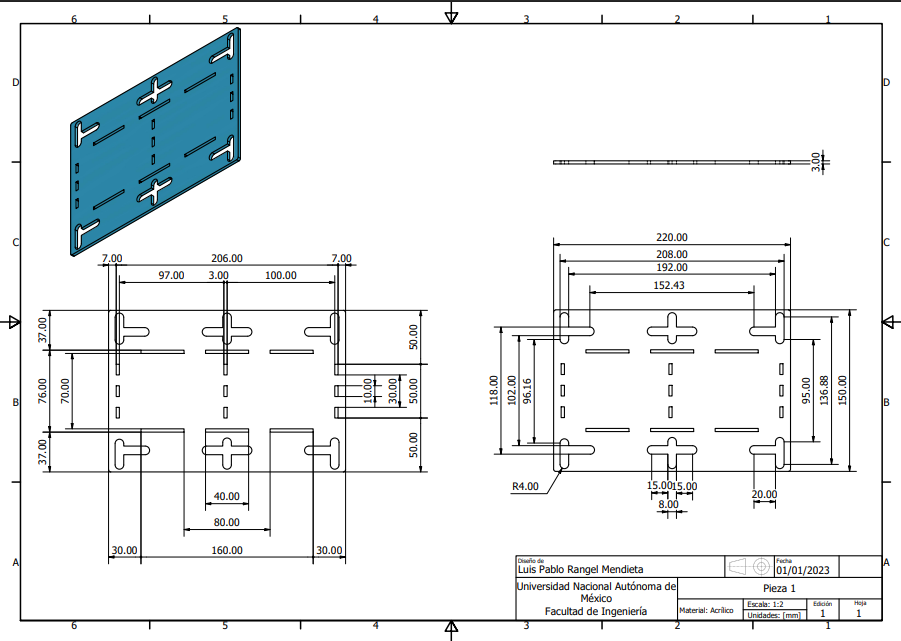
\includegraphics[width=\textwidth]{base}
    \caption{Base (pieza 1).}
    \label{fig:plano_base}
  \end{subfigure}
  \hfill
  \begin{subfigure}[b]{0.48\textwidth}
    \centering
    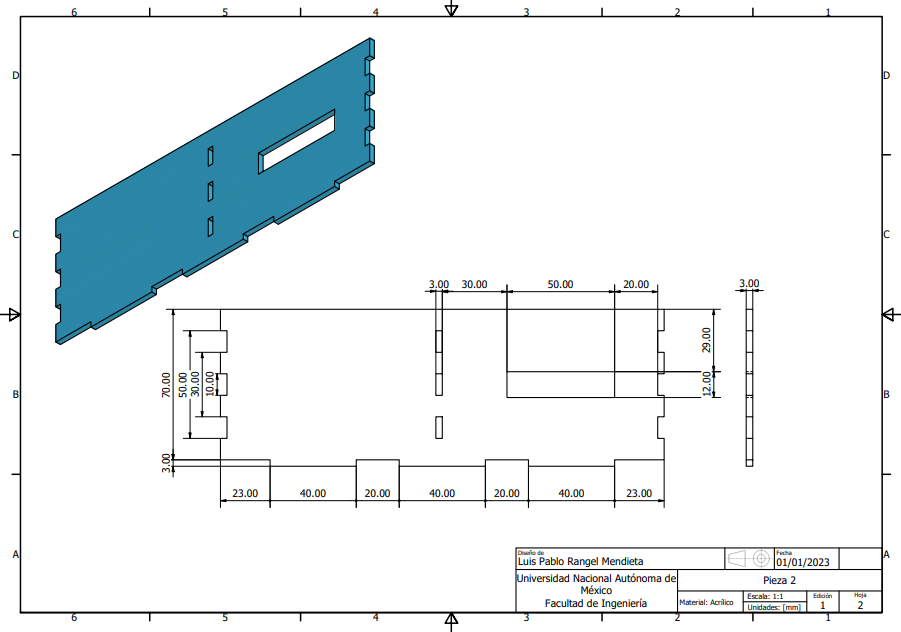
\includegraphics[width=\textwidth]{pared_laser_entrada}
    \caption{Pared larga con la ranura de la ventana de cuarzo (pieza 2).}
    \label{fig:plano_pared_laser}
  \end{subfigure}

  \vspace{1em}

  \begin{subfigure}[b]{0.32\textwidth}
    \centering
    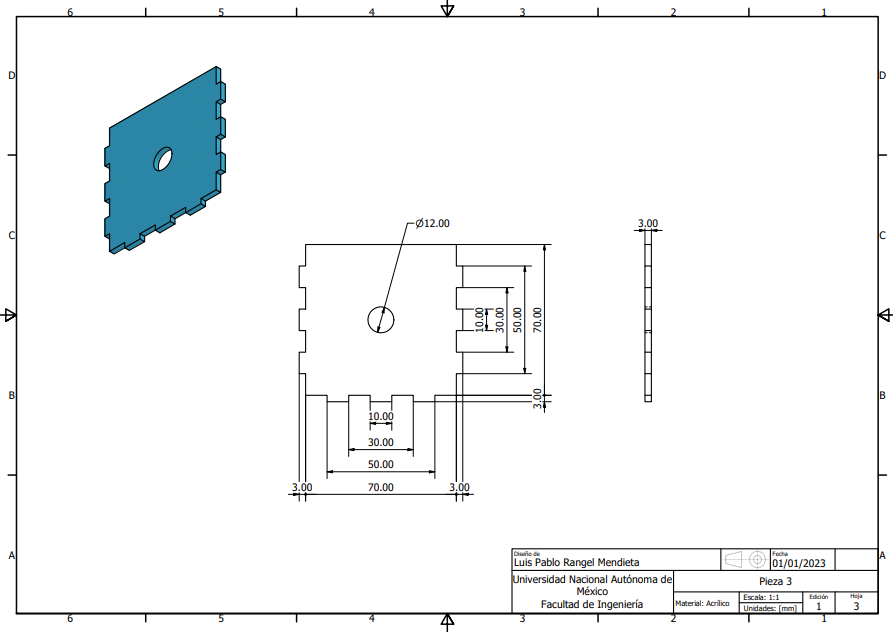
\includegraphics[width=\textwidth]{pared_hidrofono}
    \caption{Cabezal, \diameter\SI{12}{\milli\meter} (pieza 3).}
    \label{fig:plano_pared_h1}
  \end{subfigure}
  \hfill
  \begin{subfigure}[b]{0.32\textwidth}
    \centering
    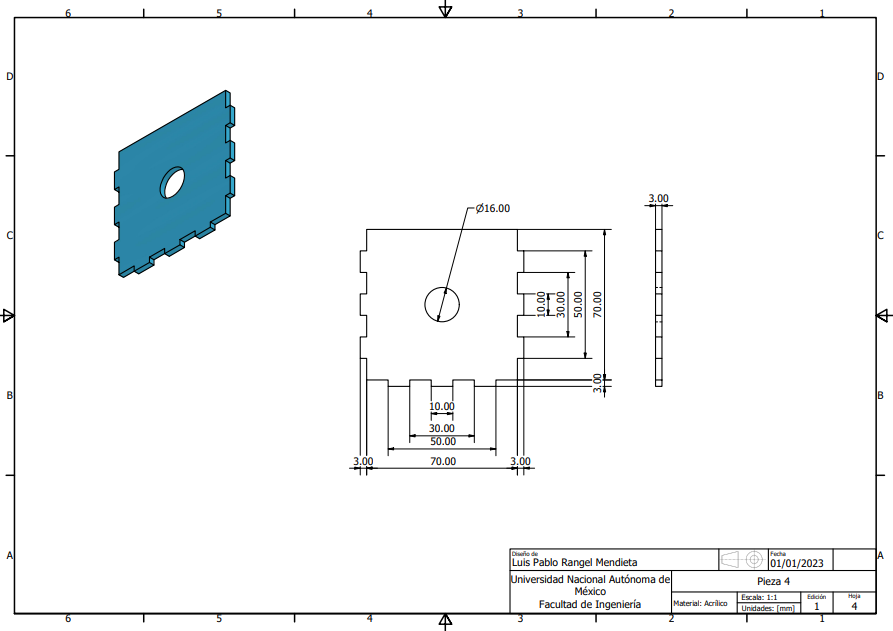
\includegraphics[width=\textwidth]{pared_hidrofono_2}
    \caption{Cuerpo, \diameter\SI{16}{\milli\meter} (pieza 4).}
    \label{fig:plano_pared_h2}
  \end{subfigure}
  \hfill
  \begin{subfigure}[b]{0.32\textwidth}
    \centering
    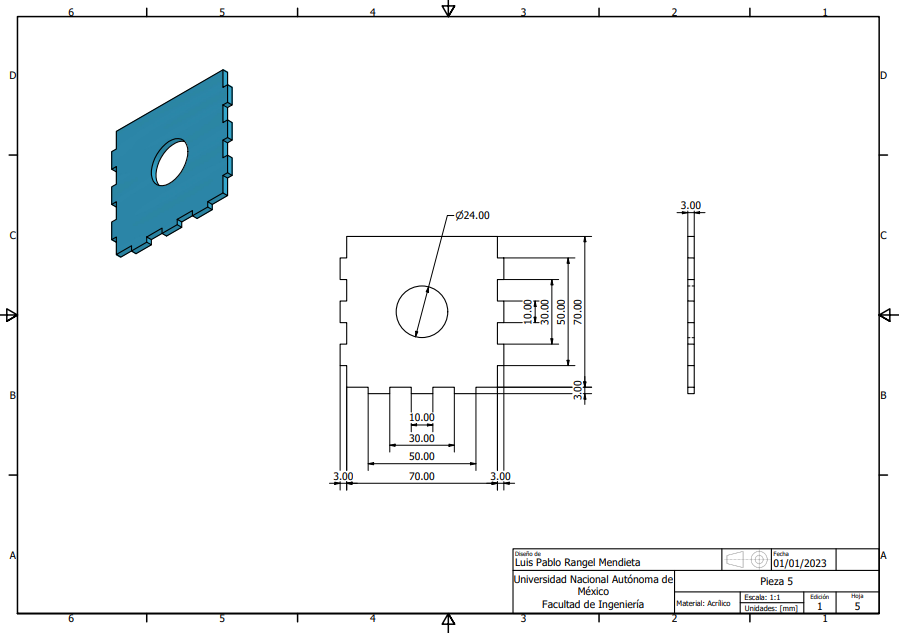
\includegraphics[width=\textwidth]{pared_hidrofono_3}
    \caption{Cable, \diameter\SI{24}{\milli\meter} (pieza 5).}
    \label{fig:plano_pared_h3}
  \end{subfigure}

  \caption{Planos de fabricación de la celda fotoacústica, en acrílico de
           \SI{3}{\milli\meter} de espesor y con cotas en milímetros. Las
           tres placas de la pared del hidrófono son coaxiales y sus
           barrenos alojan sucesivamente el cabezal, el cuerpo y el cable
           del transductor, de modo que su eje se mantenga perpendicular
           al del haz. Tomados de Rangel Mendieta \cite{Rangel2023}.}
  \label{fig:planos_celda}
\end{figure}

\section*{Hipótesis geométricas}

El cálculo descansa en cuatro suposiciones, todas ellas consecuencia de
la construcción de la celda descrita en la \cref{sec:celda}.

La primera es que la región iluminada se comporta como una fuente
lineal. El haz atraviesa la cavidad a lo largo de su ancho interno,
aproximadamente \SI{70}{\milli\meter} según la \cref{fig:planos_celda},
con un diámetro mucho menor, de
modo que la columna de líquido excitada es larga y delgada y emite una
onda cilíndrica en el plano perpendicular a su eje. El problema se
reduce así a dos dimensiones: basta considerar la sección transversal
que contiene al hidrófono.

La segunda es que la cara sensora del hidrófono se encuentra a una
distancia $d$ del eje del haz, medida perpendicularmente a él. Las tres
placas coaxiales de la pared del hidrófono ---con barrenos de
\SI{12}{\milli\meter}, \SI{16}{\milli\meter} y \SI{24}{\milli\meter}
para el cabezal, el cuerpo y el cable respectivamente--- mantienen el
eje del transductor perpendicular al del haz, condición que permite
tratar $d$ como una distancia única y no como una función de la
posición a lo largo del transductor.

La tercera es que las reflexiones en la superficie libre y en el fondo
son especulares. Ambas fronteras separan medios de impedancia acústica
muy distinta ---agua y aire en un caso, agua y acrílico en el otro---,
de modo que la reflexión es prácticamente total y puede representarse
mediante una fuente imagen situada simétricamente respecto de la
frontera. La trayectoria reflejada es entonces la recta que une la
fuente imagen con el receptor.

La cuarta es que la velocidad del sonido en el líquido es uniforme.
Para agua a \SI{20}{\celsius} se toma
$v = \SI{1480}{\meter\per\second}$.

La \cref{fig:celda_corte} reúne las cuatro hipótesis en el plano sobre
el que se resuelve el problema.

% ------------------------------------------------------------
%  Corte de la celda fotoacústica en el plano que contiene al
%  hidrófono. Cotas en milímetros. La escala vertical está
%  exagerada respecto de la horizontal para dar legibilidad a
%  las alturas, que son pequeñas frente a la longitud.
% ------------------------------------------------------------
\begin{figure}[H]
  \centering
  \begin{tikzpicture}[x=0.042cm, y=0.11cm, line join=round]

    % --- parámetros geométricos -----------------------------
    \def\Largo{200}      % longitud interna de la cavidad
    \def\Alto{70}        % altura interna de la cavidad
    \def\Espesor{3}      % espesor del acrílico
    \def\Tirante{28.6}   % tirante de líquido
    \def\Hhaz{20.5}      % altura del eje del haz sobre el fondo
    \def\Xhaz{55}        % posición del haz a lo largo de la celda
    \def\Dh{85}          % separación dibujada entre haz e hidrófono

    % --- líquido --------------------------------------------
    \fill[blue!12] (0,0) rectangle (\Largo,\Tirante);

    % --- paredes de acrílico --------------------------------
    \fill[black!25]
      (-\Espesor,-\Espesor) rectangle (0,\Alto);
    \fill[black!25]
      (\Largo,-\Espesor) rectangle (\Largo+\Espesor,\Alto);
    \fill[black!25]
      (-\Espesor,-\Espesor) rectangle (\Largo+\Espesor,0);

    % --- contorno de la cavidad -----------------------------
    \draw[thick] (0,\Alto) -- (0,0) -- (\Largo,0) -- (\Largo,\Alto);

    % --- superficie libre -----------------------------------
    \draw[blue!60, thick] (0,\Tirante) -- (\Largo,\Tirante);

    % --- trayectorias acústicas -----------------------------
    \draw[red!70!black, thick]
      (\Xhaz,\Hhaz) -- (\Xhaz+\Dh,\Hhaz);
    \draw[red!70!black, dashed]
      (\Xhaz,\Hhaz) -- (\Xhaz+0.5*\Dh,\Tirante)
                    -- (\Xhaz+\Dh,\Hhaz);
    \draw[red!70!black, dashed]
      (\Xhaz,\Hhaz) -- (\Xhaz+0.5*\Dh,0)
                    -- (\Xhaz+\Dh,\Hhaz);

    % --- haz visto de punta ---------------------------------
    \fill[orange!80!black] (\Xhaz,\Hhaz) circle (1.6mm);
    \draw (\Xhaz,\Hhaz) circle (1.6mm);

    % --- hidrófono ------------------------------------------
    \fill[black!70]
      (\Xhaz+\Dh,\Hhaz-5) rectangle (\Xhaz+\Dh+11,\Hhaz+5);

    % --- ranura de la ventana de cuarzo ---------------------
    \draw[violet, very thick] (-\Espesor,12) -- (-\Espesor,29);

    % --- cotas verticales -----------------------------------
    \draw[<->] (\Largo+14,0) -- (\Largo+14,\Tirante)
      node[midway, right=1pt] {\scriptsize $H = \SI{28.6}{\milli\meter}$};
    \draw[<->] (\Xhaz-22,0) -- (\Xhaz-22,\Hhaz)
      node[midway, left=1pt] {\scriptsize $h_f$};
    \draw[<->] (\Xhaz-22,\Hhaz) -- (\Xhaz-22,\Tirante)
      node[midway, left=1pt] {\scriptsize $h_s$};

    % --- cota horizontal ------------------------------------
    \draw[<->] (\Xhaz,-11) -- (\Xhaz+\Dh,-11)
      node[midway, below=1pt] {\scriptsize $d$};
    \draw[dotted] (\Xhaz,\Hhaz) -- (\Xhaz,-11);
    \draw[dotted] (\Xhaz+\Dh,\Hhaz) -- (\Xhaz+\Dh,-11);

    % --- rótulos --------------------------------------------
    \node[anchor=west, font=\scriptsize]
      at (\Xhaz+\Dh+12,\Hhaz) {hidrófono};
    \node[anchor=south, font=\scriptsize]
      at (\Xhaz-9,\Hhaz+3) {haz};
    \node[anchor=east, font=\scriptsize, align=right]
      at (-6,20.5) {ranura de la\\ventana};
    \node[anchor=west, font=\scriptsize, text=blue!60!black]
      at (4,\Tirante+4) {superficie libre};

  \end{tikzpicture}
  \caption{Corte de la celda en el plano que contiene al hidrófono. El
           haz se ve de punta, a la altura $h_f$ sobre el fondo que fija
           la ranura de la ventana de cuarzo. La separación $d$ entre el
           eje del haz y la cara sensora se mide en cada sesión. Las
           líneas punteadas son las trayectorias de las primeras
           reflexiones en la superficie libre y en el fondo. La escala vertical está
           exagerada respecto de la horizontal.}
  \label{fig:celda_corte}
\end{figure}


\section*{Posición del haz dentro de la cavidad}

La altura del haz sobre el fondo no es un parámetro libre: la fija la
ranura que aloja la ventana de cuarzo en la pared larga, que abarca de
\SI{12}{\milli\meter} a \SI{29}{\milli\meter} medidos desde el fondo.
El haz atraviesa el centro de esa ranura, de modo que su altura sobre
el fondo es

\begin{equation}
    h_f = \frac{\SI{12}{\milli\meter} + \SI{29}{\milli\meter}}{2}
        = \SI{20.5}{\milli\meter}.
    \label{eq:altura_haz}
\end{equation}

La distancia del haz a la superficie libre se obtiene restando esa
altura al tirante de líquido establecido en la \cref{eq:tirante}:

\begin{equation}
    h_s = H - h_f = \SI{28.6}{\milli\meter} - \SI{20.5}{\milli\meter}
        = \SI{8.1}{\milli\meter}.
    \label{eq:altura_superficie}
\end{equation}

Conviene notar que $h_s$ depende del volumen vertido y $h_f$ no. El
llenado desplaza la superficie libre; la ventana de cuarzo permanece
donde está.

\section*{Trayectorias}

Con la fuente lineal a distancia $d$ del hidrófono y a alturas $h_s$ y
$h_f$ de las fronteras horizontales, las longitudes de las
trayectorias son las siguientes.

La señal directa recorre la distancia que separa la columna iluminada
del transductor:

\begin{equation}
    \ell_{\text{dir}} = d.
    \label{eq:traj_directa}
\end{equation}

La reflexión en la superficie libre se construye colocando una fuente
imagen a una altura $h_s$ por encima de la superficie, es decir, a
$2h_s$ de la fuente real. La trayectoria es la hipotenusa del triángulo
rectángulo cuyos catetos son $d$ y $2h_s$:

\begin{equation}
    \ell_{\text{sup}} = \sqrt{d^{2} + (2h_s)^{2}}.
    \label{eq:traj_superficie}
\end{equation}

La reflexión en el fondo se obtiene de forma análoga con la fuente
imagen a $2h_f$:

\begin{equation}
    \ell_{\text{fondo}} = \sqrt{d^{2} + (2h_f)^{2}}.
    \label{eq:traj_fondo}
\end{equation}

Las reflexiones en las paredes transversales de la celda ocurren a una
distancia del orden de la mitad de la longitud interna de la cavidad,
aproximadamente \SI{100}{\milli\meter}. Su arribo es tan posterior al
de las anteriores que basta acotarlo: no compite con la ventana útil,
pero sí fija el límite superior de la longitud de registro que tiene
sentido conservar.

El tiempo de arribo de cada trayectoria es su longitud dividida entre
la velocidad del sonido:

\begin{equation}
    t = \frac{\ell}{v}.
    \label{eq:tiempo_arribo}
\end{equation}

\section*{Evaluación para la geometría nominal}

Tomando el valor nominal $d = \SI{10}{\milli\meter}$ reportado por
Rangel Mendieta \cite{Rangel2023}, junto con
$h_f = \SI{20.5}{\milli\meter}$, $h_s = \SI{8.1}{\milli\meter}$ y
$v = \SI{1480}{\meter\per\second}$, las
\crefrange{eq:traj_directa}{eq:tiempo_arribo} producen los valores de
la \cref{tab:tiempos_celda}: \SI{10.0}{\milli\meter} y
\SI{6.8}{\micro\second} para la señal directa,
\SI{19.0}{\milli\meter} y \SI{12.9}{\micro\second} para la reflexión
en la superficie libre, \SI{42.1}{\milli\meter} y
\SI{28.5}{\micro\second} para la reflexión en el fondo, y
aproximadamente \SI{100}{\milli\meter} y \SI{67.6}{\micro\second} para
las paredes transversales.

La ventana temporal libre de reflexiones es la diferencia entre los dos
primeros arribos:

\begin{equation}
    \Delta t = \frac{\sqrt{d^{2} + (2h_s)^{2}} - d}{v}
             \approx \SI{6.1}{\micro\second}.
    \label{eq:ventana_util}
\end{equation}

\section*{Dependencia respecto del montaje}

El láser es un recurso compartido y la celda no se encuentra fijada de
manera permanente a la mesa óptica, de modo que la geometría del
arreglo se restablece al inicio de cada sesión. En consecuencia, $d$ no
es una constante del sistema sino un parámetro del montaje del día, y
los valores anteriores corresponden a la geometría nominal, no a una
propiedad invariante de la celda.

La \cref{eq:ventana_util} muestra que la ventana útil se acorta al
aumentar $d$. Con el hidrófono a \SI{5}{\milli\meter} del haz la
ventana se extiende a aproximadamente \SI{8.1}{\micro\second}; a
\SI{15}{\milli\meter} se reduce a cerca de \SI{4.8}{\micro\second}. La
diferencia no es despreciable frente a la duración del pulso bipolar
que se pretende resolver, por lo que la base de tiempo y la longitud de
registro configuradas en el osciloscopio deben verificarse contra la
geometría efectiva de cada sesión y no darse por heredadas.

El procedimiento para hacerlo consta de tres pasos. Primero, medir con
vernier la separación entre la cara sensora del hidrófono y el eje del
haz, lo que proporciona $d$. Segundo, confirmar el volumen vertido, que
mediante la \cref{eq:tirante} determina el tirante $H$ y con él la
altura $h_s$ de la \cref{eq:altura_superficie}; la altura $h_f$ no
requiere verificación, pues la fija la ranura de la ventana de cuarzo.
Tercero, evaluar la \cref{eq:ventana_util} con esos valores y comparar
el resultado con la base de tiempo configurada.

Ninguna de estas dos magnitudes se registra actualmente en los
metadatos de sesión. Su incorporación al formato descrito en la
\cref{sec:formato_datos} se plantea en el \cref{cap:conclusiones} como
mejora pendiente: mientras no se registren, la reconstrucción posterior
de la ventana útil de una sesión depende de la bitácora del operador y
no del archivo de datos.


\end{document}
